\section{Problem 5}
Given the following state space model:
\begin{align*}
x_t &= \phi x_{t-1} + w_t & w_t &\sim N(0, \sigma_w^2) \\
y_t &= x_t + v_t & v_t &\sim N(0, \sigma_v^2)
\end{align*}
With the initial distribution is given by $x_0 \sim N(0, \sigma^2_w/(1-\phi^2))$.
\subsection{Matching the autocorrelation function to an ARMA(1,1) }
First we find the autocovariance function $\gamma'(h)$ of a general causal ARMA(1,1) model:
\begin{equation}
y_t = \phi' y_{t-1} + \theta' w'_{t-1} + w'_t \qquad w'_t \sim N(0, \sigma^2_{w'})
\end{equation}

Here I use the symbols $\gamma'(h)$, $\phi'$, $\theta'$ and $w'_t$ to distinguish with the similar symbols using by the state space model. Multiplying both sides of the ARMA(1,1) equation by $y_{t-h}$ and take the expectation, we can derive the difference equation for $\gamma'(h)$:

\begin{equation}
E(y_ty_{t-h}) = \phi' E(y_{t-1}y_{t-h}) + \theta' E(w_{t-1} y_{t-h}) + E(w'_t y_{t-h})
\end{equation}
\begin{equation}
\Leftrightarrow \gamma'(h) = \phi' \gamma'(h-1) + \theta' E(w_{t-1} y_{t-h}) + E(w'_t y_{t-h})
\end{equation}

Using the causality assumption: $E(w'_t y_s) = 0$ when $t > s$, we can easily derive the difference equation of $\gamma'(h)$:
\begin{equation} \label{eq:diff_gamma'}
\gamma'(h) = \phi' \gamma'(h-1) \qquad \qquad (h\geq 2)
\end{equation}
 with initial conditions:
\begin{align*}
\gamma'(0) &= \phi'\gamma'(1) + (1+\theta'\phi'+\theta'^2)\sigma^2_{w'} &  (h &= 0) \\
\gamma'(1) &= \phi'\gamma'(0) + \theta'\sigma^2_{w'}  & (h &= 1)
\end{align*}
which can be easily solved to:
\begin{equation}
\begin{split}
\gamma'(0) &= \sigma^2_{w'} \frac{(1+\theta'\phi')(\phi'+\theta')}{1-\phi'^2} \\
\gamma'(1) &= \sigma^2_{w'} \frac{1+2\theta'\phi'+\theta'^2}{1-\phi'^2}
\end{split}
\end{equation}
Since the difference equation (\ref{eq:diff_gamma'}) has one real root $z_0 = \frac{1}{\phi'}$, the general solution must be in the form $\gamma'(h) = c \phi'^h$ for $h \geq 1$. Therefore $c = \frac{\gamma'(1)}{\phi'}$

Using the initial conditions, we now have the following equations that can fully describe the autocorrelation function of the ARMA(1, 1) model: 
\begin{equation} \label{eq:ARMA11_acf}
\begin{split}
\gamma'(h) &= \sigma^2_{w'} \frac{(1+\theta'\phi')(\phi'+\theta')}{1-\phi'^2} \phi'^{h-1} \qquad (h \geq 1) \\
\gamma'(0) &= \sigma^2_{w'} \frac{1+2\theta'\phi'+\theta'^2}{1-\phi'^2} \\
\end{split}
\end{equation}

Now we derive the autocorrelation function $\gamma(h)$ for the given state space model.
\begin{equation} \label{eq:statespace_acf_half}
\begin{split}
	y_t &= x_t + v_t \\
\Leftrightarrow E(y_ty_{t-h}) &= E(x_t y_{t-h}) + E(v_t y_{t-h})\\
\Leftrightarrow \gamma(h) &= E(x_t (x_{t-h}+v_{t-h})) + E(v_t y_{t-h}) \\
\Leftrightarrow \gamma(h) &= \gamma_x(h) + E(v_t y_{t-h}) 
\end{split}	
\end{equation}
First we  must find $\gamma_x(h)$, which is the autocovariance function of $x_t$. Since $x_t$ is a causal $AR(1)$ process, the difference equation of its autocovariance function can be derived as:
\begin{equation}
\begin{split}
	x_t &= \phi x_{t-1} + w_t \\
\Leftrightarrow E(x_tx_{t-h}) &= \phi E(x_{t-1}x_{t-h})+E(w_t x_{t-h})\\
\Leftrightarrow \gamma_x(h) &= \phi \gamma_x(h-1) +E(w_t x_{t-h})
\end{split}
\end{equation} 
Using the causality, we get the following difference equation with initial condition:

\begin{align*}
\gamma_x(h) &= \phi \gamma_x(h-1) & (h &\geq 1) \\
\gamma_x(0) &= \phi \gamma_x(1) + \sigma^2_w & (h &= 0)\\
\gamma_x(1) &= \phi \gamma_x(0) & (h &= 1)
\end{align*}
The initial condition can easily be solved to:
\begin{equation}
\begin{split}
\gamma_x(0) &= \frac{\sigma^2_w}{1-\phi^2} \\
\gamma_x(1) &= \frac{\phi\sigma^2_w}{1-\phi^2}
\end{split} 
\end{equation}
Since the difference equation has only one real root $z_0 = \frac{1}{\phi}$, its general solution has the form $\gamma_x(h) = c \phi^{h}$ when $h \geq 1$. Therefore $c = \frac{\gamma_x(1)}{\phi} = \frac{\sigma_w^2}{1-\phi^2}$

This leads to the general autocovariance function of AR(1):
\begin{equation}
\gamma_x(h) = \frac{\sigma_w^2}{1-\phi^2} \phi^h
\end{equation}

Replace this to (\ref{eq:statespace_acf_half}), and use the causality property of $y_t$, we get the covariance function of the given state space model:

\begin{equation} \label{eq:statespace_acf}
\begin{split}
\gamma(h) &= \frac{\sigma_w^2}{1-\phi^2}\phi^h  \qquad \qquad (h \geq 1)\\
\gamma(0) &= \frac{\sigma_w^2}{1-\phi^2} + \sigma_v^2
\end{split}
\end{equation}

By matching the above $\gamma(h)$ and $\gamma(0)$ to $\gamma'(h)$ and $\gamma'(0)$ given in (\ref{eq:ARMA11_acf}), we can then express the given state space model in an ARMA(1,1) form. This leads to the following conditions:
\begin{equation}\label{eq:ARMA_11_conditions}
\begin{split}
\frac{\sigma_w^2}{1-\phi^2}\phi^h &= \sigma^2_{w'} \frac{(1+\theta'\phi')(\phi'+\theta')}{1-\phi'^2}\phi'^{h-1} \qquad (h \geq 1) \\
\frac{\sigma_w^2}{1-\phi^2} + \sigma_v^2 &= \sigma^2_{w'} \frac{1+2\theta'\phi'+\theta'^2}{1-\phi'^2} 
\end{split}
\end{equation}

We can also see that $\phi'= \phi$, otherwise the first condition can not be satisfied for all $h \geq 1$. We can then simplify the condition to the following form:

\begin{equation}\label{eq:ARMA_11_simp_conds}
\begin{split}
\sigma^2_{w'}(1+\theta'\phi)(\phi+\theta') &= \phi\sigma_w^2 \\
\sigma^2_{w'}(1+2\theta'\phi+\theta'^2) &= \sigma_w^2+ (1-\phi^2) \sigma_v^2
\end{split}
\end{equation}
\subsection{Find the parameters for invertible ARMA(1,1) model}
\subsubsection{Case 1: $\phi = 0.5, \sigma_w^2 = 1, \sigma_v^2 = 2$}
To find the parameter of the corresponding invertible ARMA(1,1), we replace $\phi$, $\sigma$ and $\sigma_v$ into (\ref{eq:ARMA_11_simp_conds}):
\begin{equation}
\begin{split}
	\sigma^2_{w'}(1+0.5\theta')(0.5+\theta') &= 0.5 \\
	\sigma^2_{w'}(1+\theta'+\theta'^2) &= 2.5
\end{split}
\end{equation}
\begin{equation}
\begin{split}
\Leftrightarrow
	\theta'^2 + 3.5\theta' + 1 &= 0\\
	\sigma^2_{w'}(1+\theta'+\theta'^2) &= 2.5
\end{split}
\end{equation}
 Since the ARMA(1,1) is invertible, we must have $|\theta'| < 1$, which leads to the following solution:
 \begin{equation} \label{eq:ARMA_11_case1}
 \begin{split}
 \theta' &\approx -0.314 \\
 \sigma_{w'}^2 &\approx 3.186
 \end{split}
 \end{equation}
\subsubsection{Case 2: $\phi = 0.5, \sigma_w^2 = 1, \sigma_v^2 = 20$}
 Replacing these assumptions into (\ref{eq:ARMA_11_simp_conds}), we have:
  \begin{equation}
  \begin{split}
  \sigma^2_{w'}(1+0.5\theta')(0.5+\theta') &= 0.5 \\
  \sigma^2_{w'}(1+\theta'+\theta'^2) &= 16
  \end{split}
  \end{equation}
  \begin{equation}
  \begin{split}
    \Leftrightarrow
    \theta'^2 + 2.6\theta'+1 = 0 \\
    \sigma^2_{w'}(1+\theta'+\theta'^2) &= 16
  \end{split}
  \end{equation}
Using the condition that $|\theta'|<1$, we get the following solution:
\begin{equation} \label{eq:ARMA_11_case2}
\begin{split}
	\theta' &\approx -0.469 \\
	\sigma^2_{w'} &\approx 21.307
\end{split}
\end{equation}
\subsection{Spectral density of the two ARMA(1, 1)}

We see that in Figure \ref{fig:SpectralDensity2ARMA}, the shape of the spectral density of the two ARMA(1,1) models are almost the same. However, the spectral density of the second case is higher than the first case by a constant factor equal to $18$ which is the difference in $\sigma^2_v$ of the two cases. This shows that, the observation noise in the state space model contributes uniformly to its spectral density. 

This effect is obvious when we look at the autocovariance function $\gamma(h)$ of the state space model given in (\ref{eq:statespace_acf}). We see that $\sigma^2_v$ only contribute to $\gamma(0)$, which will become an addictive constant when we apply the transform $f(\omega) = \sum_{h = -\infty}^{\infty} \gamma(h) e^{-2 \pi i \omega h}$.

\begin{figure}
	\centering
	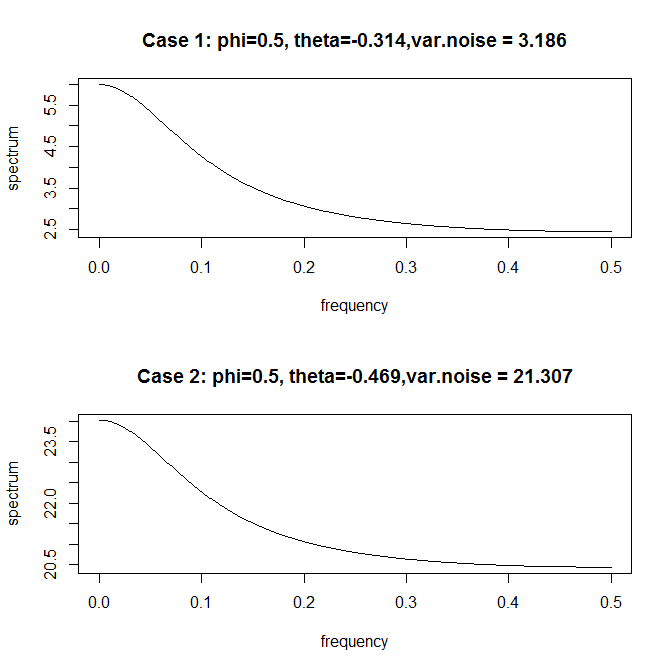
\includegraphics[width=10cm]{Figures/Problem5_1}
	\caption{Theoretical spectral density of the two ARMA(1,1) models}
	\label{fig:SpectralDensity2ARMA}
\end{figure}

\subsection{Simulating and Estimating the Spectra of two cases}
The simulation of 200 observations of the two ARMA(1,1) models is given in Figure \ref{fig:Simulation}. Their estimated spectra is given in Figure \ref{fig:EstimateSpectra}. I used the averaged periodogram as the smoothing method, with $L = 9$.

\begin{figure}
	\centering
	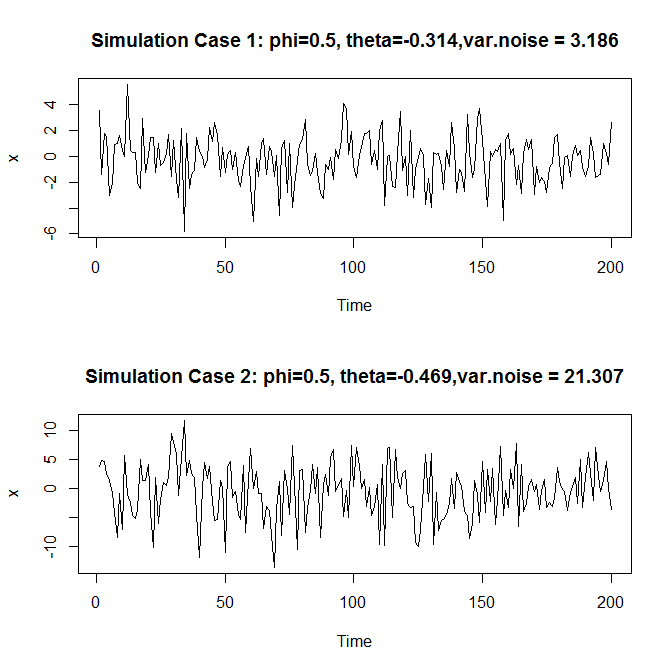
\includegraphics[width=9cm]{Figures/Problem5_2}
	\caption{Simulation of 200 observations of the two ARMA(1,1) models}
	\label{fig:Simulation}
\end{figure}

\begin{figure}
	\centering
	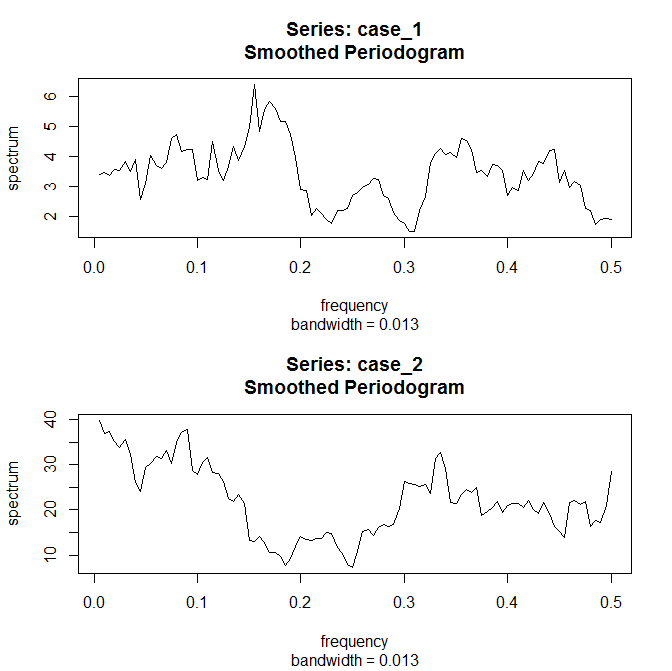
\includegraphics[width=9cm]{Figures/Problem5_3}
	\caption{Estimated spectra of the two ARMA(1,1) models, using averaged periodograms with $L=9$}
	\label{fig:EstimateSpectra}
\end{figure}
